\chapter{Diseño e implementación} % Main chapter title

\label{Chapter3} % Change X to a consecutive number; for referencing this chapter elsewhere, use \ref{ChapterX}

%--------------------------------------------------------------------------------------
\section{Descripción del sistema}

El \textit{SAL/T}, según sus siglas, Sistema de Aislamiento Limitado o Total \citep{salt-physical-paper}, es un sistema que le permite al conductor la activación y desactivación del modo aislado limitado. En este modo, el equipo permite la circulación de la formación al desactivar las señales de corte de tracción y freno de emergencia generadas por los otros subsistemas. Para que esta operación se realice de forma segura, se debe monitorear la velocidad de la formación tal que sea posible evitar que supere cierto valor máximo. Se considera un sistema crítico debido a que, en caso de fallar, puede ocasionar lesiones o muertes de personas, dañar el medio ambiente y/o generar grandes pérdidas materiales.

En trabajos anteriores se han desarrollado las primeras cinco fases de catorce que componen el ciclo de vida según la norma \textit{UNE-EN 50126}, centradas en el relevamiento de la necesidad y la obtención de los requerimientos técnicos del sistema.

En esta oportunidad, tal como se puede observar en el margen inferior derecho de la figura 1, se plantea el desarrollo de una central operativa. Se trata de una plataforma web que cuenta con una unidad lógica de compartición y empaquetado de software posibilitando la administación, la configuración y el monitoreo en tiempo real de la información recibida y transmitida por parte de cada dispositivo \textit{SAL/T}. 

En caso de ser necesario, a partir de la activación de una señal crítica provista por el artefacto \textit{Hasler} \footnote{ Es un sistema electromecánico que registra los eventos de velocidad del material rodante, la señal de anuncio y la señal de frenado automático.
}  que se encuentra instalado en cada formación ferroviaria, un operario puede accionar alguno de los comandos que se listan a continuación:


\begin{itemize}
	\item \textbf{Modo aislado total}: se habilita la tracción y se libera el freno de emergencia, independientemente de cualquier condición. 

    \item \textbf{Modo coche en deriva}: se corta la tracción y se libera el freno de emergencia, independientemente de cualquier condición. 

    \item \textbf{Modo parada total}: se corta la tracción y se aplica el freno de emergencia, independientemente de cualquier condición. 
    
    \item \textbf{Modo intermitente}: se habilita la tracción y se aplica el freno de emergencia en ciclos de tiempo configurables. 

    \item Anulación de comandos remotos vigentes.

\end{itemize}


Para el seguimiento de las variables, publicadas por cada dispositivo \textit{SAL/T}, que permiten la visualización en la plataforma, se realiza la suscripción a un tópico del \textit{broker} \textit{MQTT} y se registra la información indexada en la base de datos de un servidor. En consecuencia, resulta de extrema importancia que la comunicación a través de \textit{MQTT} opere sobre el protocolo de encriptación \textit{SSL/TSL}, de modo que se exponga un considerable nivel de seguridad; de igual manera, es necesaria la utilización de certificados para el acceso a la lectura y la escritura en la base de datos.  

Así mismo, la página web ofrece la configuración de los parámetros de cada dispositivo conectado a la formación ferroviaria, la administración de los roles y la autenticación de los usuarios.

\begin{figure}[htpb]
\centering 
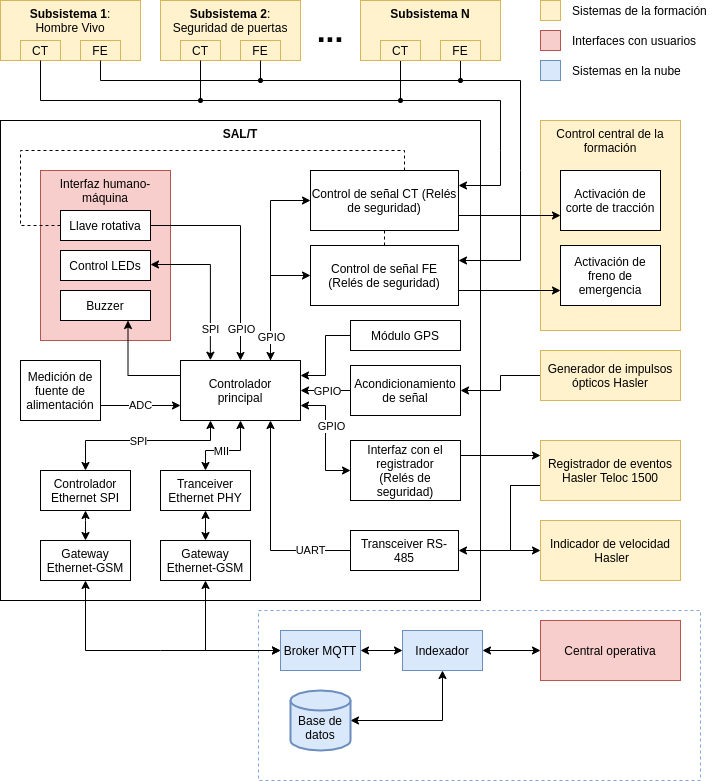
\includegraphics[width=.8\textwidth]{Figures/diagrama_salt_con_central.png}
\caption{Diagrama en bloques del sistema SALT.}
\label{fig:diagBloques}
\end{figure}


%--------------------------------------------------------------------------------------
\newpage
\section{Arquitectura del sistema}

En este apartado se ahonda en la estratificación del \textit{stack IoT}, como se puede ver en la figura \ref{fig:salt-architecture}, que se compone de varias capas que cumplen funciones específicas en el ámbito de los sistemas \textit{IoT}. Se analiza, de este modo, cómo se relacionan las diferentes tecnologías que se utilizan en cada capa, y cómo se aprovechan estas interacciones para obtener soluciones integral y escalable. 


\begin{figure}[htpb]
  \centering 
  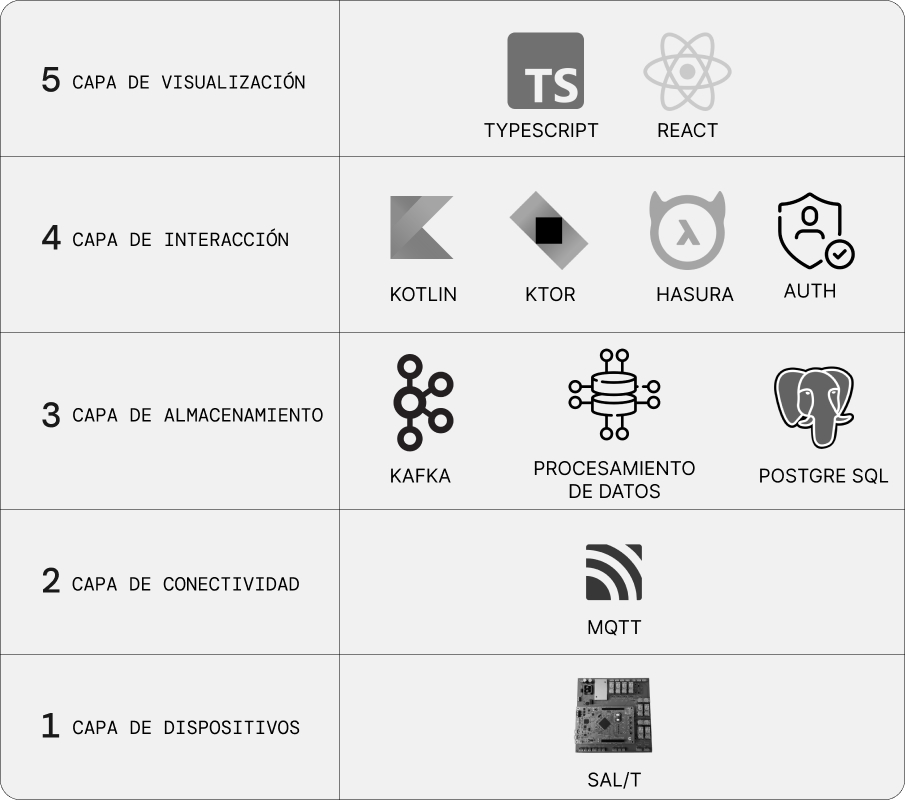
\includegraphics[width=.75\textwidth]{Figures/cuadro.jpg}
  \caption{Arquitectura de la Central Operativa SAL/T.}
  \label{fig:salt-architecture}
\end{figure}


\subsection{Capa de dispositivos}

Sobre la base de un prototipo del Sistema de Aislamiento Limitado o Total, \textit{SAL/T}, se desarrolló mediante el kit de desarrollo \textit{Nucleo F429} \citep{nucleo-kit}, un cliente \textit{MQTT} que permite la publicación de la velocidad de la formación y de los parámetros provistos por los subsistemas de falla, entre otras variables; y llegado el caso, el dispositivo pueda realizar la lectura de diferentes parámetros configurables.


\subsection{Capa de conectividad}

Para la comunicación entre los dispositivos \textit{SAL/T} y la capa de almacenamiento se emplea un \textit{Broker MQTT} que oficia de orquestador entre el cliente, el dispositivo \textit{SAL/T} que publica los mensajes y \textit{Apache Kafka}, un sistema distribuido que efectúa la lectura de la información y su posterior procesamiento. 

Dado que los mensajes intercambiados entre las partes contienen información sensible, se ha optado por agregar la capa de seguridad \textit{TLS}. En este sentido, resulta indispensable utilizar el certificado \textit{X509} para prevenir ataques del tipo \textit{adversary-in-the-middle} y los certificados emitidos por autoridades reconocidas.


\subsection{Capa de almacenamiento}

La capa de almacenamiento se encuentra constituida por el sistema distribuido \textit{Kafka} que se encarga de almacenar los datos de la aplicación. Entre ellos se destacan los mensajes \textit{MQTT} enviados por los dispositivos \textit{SAL/T}, como también la información referida a las formaciones y a los \textit{SAL/T} que las ocupan. Además, se tienen servicios de procesamiento de datos que se encargan de adaptar la información de los tópicos en datos que posteriormente serán consumidos por los servicios que integran la capa superior.

Por otro lado, se tiene una base de datos relacional \textit{PostgreSQL} para el almacenamiento de los datos provenientes del servicio de autenticación y el motor que facilita la interacción con la plataforma web. Los conectores se encargan de insertar los datos que se quieran disponer a la capa de visualización.

En la figura \textbf{devicesTrainEntity} se observa el modelo de datos que representa a los dispositivos \textit{SAL/T}, las formaciones y las entidades. 
El primero cuenta con un identificador del dispositivo en el sistema, el estado de operación y una referencia al tren en el que se desplegó el artefacto. 
El modelo de la formación está enriquecido con la entidad a la que pertenece y el número de serie del tren. 
Por último, las entidades están compuestas por nombre y descripción.
En la figura \textbf{devicesSubsystems} se aprecian los subsistemas de fallas relacionados con el dispositivo \textit{SAL/T}. Su modelo está integrado con el nombre del subsistema, el identificador del dispositivo al que está asociado y el estado actual del mismo. 


\subsection{Capa de interacción}

La capa de interacción se encuentra conformada por tres unidades. Por un lado, se ha desarrollado en el lenguaje \textit{Kotlin} en conjunto con el \textit{framework} \textit{Ktor}, un microservicio de autenticación donde es posible la gestión de los usuarios con sus respectivos roles y también el \textit{backend}. Entre sus tareas principales se encuentran las relacionadas con el protocolo \textit{MQTT} para la actualización de los certificados que brindan seguridad a las comunicaciones, mediante el uso de la capa de seguridad \textit{TLS}, y la indexación de los eventos que se publiquen en tiempo real; como la configuración general que permite el funcionamiento integral de los servicios y módulos dispuestos en el sistema. \\

Además, se dispone del motor \textit{Hasura}, el cual se encuentra conectado a una base de datos relacional (\textit{PostgreSQL}) basado en el lenguaje de consulta estructurado \textit{SQL}, que permite exponer una \textit{API GraphQL} a aquellos clientes que deseen obtener una visualización del modelo de datos propuesto en que se conjuga la información de cada formación ferroviaria con su correspondiente dispositivo \textit{SAL/T} y diseño destinado al \textit{frontend}. Más aún, el enlace permite realizar modificaciones y hasta remociones de las columnas propuestas en las tablas de cada esquema dentro de la base de datos.


\subsection{Capa de visualización}

En esta capa se ha utilizado el lenguaje de programación \textit{TypeScript} junto con la biblioteca gráfica \textit{React} para brindar una web reactiva en la que se elaboraron los formularios, las tablas y los paneles a partir de la explotación de la información almacenada en la base de datos. Cabe destacar que la plataforma web se encuentra condicionada por el rol y la entidad a la que pertenece cada usuario, de modo que, cada formación ferroviaria tendrá un operador asignado, el cual podrá modificar los parámetros correspondientes con el dispositivo asociado.

En la figura \textbf{dashboard} se puede apreciar el panel de control de la central operativa al que tendrán acceso los operadores de cada entidad.
En el mismo se observan distintas tarjetas con el estado de cada subsistema de fallas y del tren, como así también un velocímetro que informa la velocidad de la formación.


%--------------------------------------------------------------------------------------
\newpage
\section{Arquitectura de datos}

La estructura de la base de datos \textit{SQL} se realiza a partir de un análisis detallado del sistema en el que se identifican las principales entidades: la formación ferroviaria, los subsistemas de falla y las áreas. Toda la información de estas entidades se nuclea en la entidad tren, la cual representa una formación ferroviaria con todos sus subsistemas y áreas asociadas. En efectp, el modelado de estas entidades y sus atributos correspondientes, se definen las relaciones entre ellas y se establecen las claves primarias y foráneas.

Para visualizar de manera más clara la estructura de la base de datos y sus relaciones, se utiliza el diagrama UML (Lenguaje de Modelado Unificado). En la siguiente figura se muestra el diagrama UML de la base de datos, donde se pueden observar las diferentes entidades, sus atributos y relaciones. A partir de este diagrama se procede a crear las tablas en la base de datos SQL y a definir sus columnas y restricciones, garantizando así la integridad de los datos y el correcto funcionamiento del sistema.


\textbf{CONTINUAR CON EL DIAGRAMA UML CONECTANDO LAS ENTIDADES  \\ VER Figures/salt\_uml\_drawio}
\url{https://app.diagrams.net/}


\subsection{Entidades del modelo de datos}
 
\subsubsection{Schema auth\_service}

\begin{itemize}

  \item \textbf{credentials}: Esta tabla almacena las credenciales de los usuarios para acceder al sistema. Tiene una clave foránea a la tabla \textbf{auth\_service users} y es referenciada por la tabla \textbf{auth\_service roles}.

  \item \textbf{roles}: Esta tabla almacena los roles de los usuarios. Tiene una clave foránea a la tabla \textbf{auth\_service users} y es referenciada por la tabla \textbf{enums roles}.

  \item \textbf{users}: Esta tabla almacena la información básica de los usuarios del sistema. Es referenciada por la tabla \textbf{auth\_service credentials} y la tabla \textbf{public users}.

\end{itemize}


\subsubsection{Schema enums}

\begin{itemize}

  \item \textbf{device status}: Esta tabla almacena los estados posibles para los dispositivos. Es referenciada por la tabla \textbf{public devices}.

  \item \textbf{events}: Esta tabla almacena los tipos de eventos posibles. Es referenciada por la tabla \textbf{public internal events}.

  \item \textbf{fail system}: Esta tabla almacena los sistemas de falla posibles. Es referenciada por la tabla \textbf{public remote events} y la tabla \textbf{public subsystems}.

  \item \textbf{roles}: Esta tabla almacena los roles posibles para los usuarios del sistema. Es referenciada por la tabla \textbf{auth\_service roles}.

\end{itemize}


\subsubsection{Schema public}

\begin{itemize}

  \item \textbf{devices}: Esta tabla almacena información sobre los dispositivos del sistema. Tiene una clave foránea a la tabla \textbf{public train} y es referenciada por la tabla \textbf{public remote events} y la tabla \textbf{public internal events}.

  \item \textbf{entities}: Esta tabla almacena información sobre las entidades del sistema. Es referenciada por la tabla \textbf{public train}.

  \item \textbf{internal events}: Esta tabla almacena información sobre los eventos internos del sistema. Tiene claves foráneas a las tablas \textbf{public devices}, \textbf{enums events} y \textbf{public users}.

  \item \textbf{remote events}: Esta tabla almacena información sobre los eventos remotos del sistema. Tiene una clave foránea a la tabla \textbf{public devices} y es referenciada por la tabla \textbf{enums fail system}.

  \item \textbf{subsystems}: Esta tabla almacena información sobre los subsistemas del sistema. Tiene una clave foránea a la tabla \textbf{public devices} y es referenciada por la tabla \textbf{enums fail system}.

  \item \textbf{train}: Esta tabla almacena información sobre los trenes del sistema. Tiene una clave foránea a la tabla \textbf{public entities} y es referenciada por la tabla \textbf{public devices}.

  \item \textbf{user data}: Esta tabla almacena información adicional de los usuarios del sistema. Es referenciada por la tabla \textbf{public users}.

  \item \textbf{users}: tabla que contiene información de los usuarios. Tiene una relación de clave externa con la tabla entities.

\end{itemize}



\section{Seguridad del sistema}

En la actualidad, la seguridad en los protocolos de comunicación es una preocupación constante en el mundo digital. Con el creciente número de amenazas cibernéticas y la sofisticación de los ataques, es esencial que los protocolos de comunicación sean lo más seguros posible. Es fundamental que los protocolos de comunicación se desarrollen y se implementen con medidas de seguridad adecuadas para garantizar la privacidad y la integridad de los datos transmitidos.


\subsection{JWT}

JWT (JSON Web Token) es un estándar de token de seguridad que se utiliza para autenticar y autorizar a los usuarios en aplicaciones web y móviles. Dentro del protocolo HTTP, JWT se utiliza como un mecanismo de autenticación para permitir el acceso seguro a recursos protegidos.

Para utilizar JWT en HTTP, primero se debe generar un token JWT en el servidor después de que el usuario se autentica correctamente. Este token se envía de vuelta al cliente como respuesta a la solicitud de autenticación.

Luego, para acceder a recursos protegidos, el cliente debe incluir el token JWT en la solicitud HTTP en la cabecera de autorización. La cabecera de autorización tiene el prefijo "Bearer" seguido del token JWT. De esta manera, el servidor puede verificar la validez del token y si el usuario tiene los permisos necesarios para acceder a la información solicitada.

Una vez que el servidor valida el token JWT y verifica que el usuario tiene los permisos necesarios, puede enviar la respuesta solicitada al cliente. Si el token no es válido o ha expirado, el servidor puede denegar el acceso al recurso solicitado.

En resumen, JWT se utiliza dentro del protocolo HTTP como un mecanismo de autenticación seguro para permitir el acceso a recursos protegidos. Al utilizar JWT, se puede evitar la necesidad de mantener una sesión persistente en el servidor y se puede compartir información de usuario entre diferentes servicios sin la necesidad de almacenarla en el servidor.


\subsection{MQTT v5.0}

En la última versión del protocolo de mensajería \textit{MQTT}, la versión 5.0, se incluyen varias mejoras en términos de seguridad en comparación con versiones anteriores, lo que lo hace más seguro y confiable para su uso en entornos \textit{IoT} y \textit{M2M}.

Una de las mejoras más importantes en \textit{MQTT v5.0} es la inclusión de un mecanismo de autenticación mejorado. Ahora, el cliente y el servidor pueden autenticarse mutuamente utilizando certificados y credenciales de usuario. Esto ayuda a prevenir ataques de suplantación de identidad y a garantizar que solo los usuarios autorizados puedan acceder al servidor \textit{MQTT}.

Otra mejora importante en \textit{MQTT v5.0} es el soporte para \textit{TLS 1.3}, la última versión del protocolo de seguridad de transporte. \textit{TLS 1.3} ofrece un cifrado más fuerte y un intercambio de claves más seguro que las versiones anteriores, lo que ayuda a proteger los datos transmitidos contra ataques de escucha y manipulación.

\textit{MQTT v5.0} también introduce la capacidad de establecer límites de tamaño máximo de paquete, lo que ayuda a prevenir ataques de inundación de paquetes que pueden afectar la disponibilidad del servidor \textit{MQTT}.

Además, la versión 5.0 de \textit{MQTT} también incluye la capacidad de definir propiedades adicionales en los mensajes \textit{MQTT}, lo que permite a los clientes y servidores intercambiar información adicional sobre los mensajes, como la hora en que se creó el mensaje o su nivel de prioridad.


%------------------------------------------------------------------------
\newpage
\section{Desarrollo del frontend}

En esta sección, se aborda la estructura de la aplicación web, incluyendo la organización de sus componentes y la relación entre ellos. Además, se analizan los diferentes roles que pueden tener los usuarios de una aplicación y cómo afectan a la funcionalidad de la misma. Por último, se describe la implementación del cliente web y los clientes que se ven involucrados en cada etapa. 


\subsection{Estructura de la aplicación web}

La estructura de la aplicación se inspira en la herramienta \textit{Create React App} \footnote{\url{https://create-react-app.dev/}}, que postula una estructura de archivos predefinida para crear aplicaciones web con React. En efecto, se plasman un conjunto de convenciones y buenas prácticas que permiten organizar el código de una forma clara y fácilmente escalable.

La organización de archivos, utilizando \textit{Typescript} y \textit{inline JSS}, consta de los siguiente elementos:

\begin{itemize}

  \item La carpeta \textit{"public"}, que contiene los archivos \textit{HTML} y otros recursos que se deben servir estáticamente al navegador.

  \item La carpeta \textit{"src"}, que es el directorio principal de la aplicación y contiene los archivos de código fuente. Dentro de esta carpeta se encuentra:

    \begin{itemize}

      \item Los archivos de configuración, como \textit{"index.tsx"} y \textit{"App.tsx"}, que se encargan de inicializar la aplicación y definir su estructura básica, utilizando la sintaxis de \textit{Typescript}.
  
      \item Los componentes de la aplicación, organizados en subdirectorios según su funcionalidad. Cada componente suele estar formado por un archivo \textit{".tsx"} en la que define su lógica y un archivo de extensión \textit{".ts"} que define el procesamiento de la información previo a su renderización.

      \item Otros recursos, como imágenes, fuentes o archivos JSON que se utilizan en la aplicación.

    \end{itemize}

  \item La carpeta \textit{"node\_modules"}, que contiene todas las dependencias de la aplicación.

  \item Los archivos \textit{"package.json"} y \textit{"package-lock.json"}, que definen la configuración y las dependencias del proyecto.

  \item Otros archivos de configuración, como \textit{".gitignore"} o \textit{".env"}, que se utilizan para personalizar la configuración de la aplicación.

\end{itemize}


\newpage
\subsection{Roles}

La aplicación web cuenta con una estructura de roles que determinan los permisos y acciones que los usuarios pueden realizar en la plataforma. En total, se establecen cuatro roles, que se listan a continuación:

\begin{itemize}

  \item \textbf{Visitante:} Este rol tiene los permisos más limitados en la plataforma y se le permite tan solo registrarse o ingresar al sistema.

  \item \textbf{Operador:} Las principales tareas del operador se centran en visualizar y/o controlar una o más formaciones ferroviarias, a través de un panel de control, asociadas a una entidad.

  \item \textbf{Supervisor:} Es aquel que asigna el \textit{SAL/T} a una formación ferroviaria y a un operador. Además, tiene el control absoluto de todas las formaciones correspondientes a una entidad.

  \item \textbf{Súper usuario:} Este es el rol con mayores permisos en la plataforma, y quien se responsabiliza de observar las tres entidades de la plataforma y a la asignación de supervisores a cada entidad, entre otras acciones disponibles en la plataforma.

\end{itemize}

Cada uno de estos roles se diseña para brindar distintos niveles de acceso y control en la plataforma, según las necesidades y responsabilidades de los usuarios en cuestión. Con esta estructura de roles, se busca garantizar la seguridad y privacidad de los datos y acciones de los usuarios.


\subsection{Modelo}


\textbf{ESCRIBIR ACERCA DEL MODELADO DE DATOS EN LA PLATAFORMA WEB - Bastian}


\subsection{Implementación de la plataforma}

La plataforma consiste en un conjunto de páginas en las que se acopla la biblioteca \textit{React Router DOM} \footnote{\url{https://reactrouter.com/en/main}}. La misma facilita la navegación y el enrutamiento de la aplicación web de una sola página. Asimismo se encuentran las ventanas emergentes que permiten realizar el alta, la baja y la modificación de cada entidad.


\subsubsection{Páginas}

Consecuentemente, se presentan las principales páginas del cliente web con su ruta y una breve descripción asociada.


\begin{itemize}

  \item Autenticación ("/auth", "/home"):
      la página de autenticación es el punto de entrada de la plataforma. De esta manera, cuando el usuario completa los formularios de registro y posteriormente de inicio de sesión, interactuando con la biblioteca \textit{JWT}, puede acceder al contenido restante del cliente web.

  \item Configuración ("/configuration"):
    la configuración del sistema permite a los usuarios ajustar las preferencias y opciones de la aplicación. En particular, se ofrece la parametrización de la conexión al broker MQTT para lograr el correcto funcionamiento de la aplicación, ya que permite la comunicación con los dispositivos que se encuentran en las formaciones ferroviarias. Por otro lado, las acciones que se encuentran disponibles en esta página se encuentran sujetas al rol de cada usuario, lo que garantiza un acceso seguro y restringido a funciones específicas de la aplicación.

  \item Áreas ("/areas", "/home"):
    Trenes Argentinos es una empresa que cuenta con tres áreas principales: cargas, infraestructura y operaciones, cada una de las cuales desempeña un papel importante en la gestión de la empresa. Desde el cliente web, los usuarios pueden acceder a cada una de estas áreas si tienen el rol correspondiente, lo que les permite realizar tareas específicas y gestionar la información relacionada con su área. Esto garantiza un acceso restringido y seguro a la información de la empresa.

  \item Usuarios ("/users"):
    contiene a todos los usuarios del ente permitiendo a los supervisores o al súper usuario tener un registro completo de los usuarios registrados y gestionar su información. Desde esta página, se puede acceder al perfile de cada usuario que se detalla a continuación. 

  \item Perfile del usuario ("/user:user-id")
    en este componente se visualizan los datos personales de cada usuarios y los eventos en los que se ve involucrado, como su ingreso en la plataforma y las acciones vinculadas a un SAL/T. 

  \item Dispositivos ("/devices")
    es una tabla que expone aa los dispositivos registrados en el sistema y su relación con las entidades y formaciones ferroviarias correspondientes. Desde esta tabla, el supervisor puede realizar el alta, baja y modificación de los dispositivos.

  \item Panel de control del dispositivo ("/control-panel:device-id")
    es una herramienta esencial en la gestión ferroviaria que dispone de múltiples funciones. Entre ellas, se encuentra un tacómetro que permite visualizar la velocidad de la formación ferroviaria en tiempo real a partir de tres fuentes de información, un componente para habilitar o deshabilitar el corte de tracción y el freno de emergencia, y una sección para visualizar los eventos al tópico en el que se encuentra suscrito vía broker MQTT.


  \item Subsistemas de falla ("/failure-subsystems:device-id")
    desde la página del panel de control, los usuarios pueden acceder fácilmente a la página de configuración de subsistemas de falla de cada tren. Esta sección es esencial para observar los sistemas asociados en caso de ocurrir una falla y llegado el caso una posible reconfiguración.

  \item Eventos ("/events:device-id")
    en caso de seleccionar el botón para expandir la fracción de página destinada a los eventos mqtt que se encuentran en el panel de control, se exhiben un listado más extenso de los eventos en tiempo real y con información más detallada. Esta funcionalidad permite una mayor capacidad de análisis y monitoreo de los eventos relacionados con la gestión ferroviaria.


\end{itemize}


\subsubsection{Ventanas emergentes}

Las vetanas emergentes se emplean para realizar el alta, baja y modificación de las entidades propuestas; como así también el modal correspondiente al igreso de contraseña de cada usuario con el que se cumple un mínimo grado de seguridad por cada acción que se realiza. 


Modales: \textit{crear: usuario, tren, dispositivo ; configuracion: sub sistemas de seguridad, etc}

modal de ingresar contraseña al realizar una acción


%------------------------------------------------------------------------
\newpage
\section{Desarrollo del backend}


A partir del uso de archivo docker-compose, que se ejecuta en un entorno Docker, para proporcionar el conjunto completo de servicios para enviar, recibir y almacenar los datos a través de diferentes protocolos. Cada servicio se ejecuta en su propio contenedor y se conecta a los otros servicios según el siguiente formato:


\textbf{AGREGAR IMAGEN DEL ENTORNO DOCKER CON SUS CONTENEDORES Y CONEXIONES }
\url{https://www.gotoiot.com/pages/articles/docker_intro/index.html}
\url{https://www.gotoiot.com/pages/articles/docker_intro/images/image2.png}


\begin{itemize}

  \item mosquitto: es un servidor MQTT de código abierto que se utiliza para enviar y recibir mensajes. Se utiliza la imagen "eclipse-mosquitto" y se mapea el puerto 1883 en el host al puerto 1883 en el contenedor. También se montan dos volúmenes, uno para la configuración del servidor y otro para los datos.

  \item hasura: es un motor de GraphQL que proporciona una API para interactuar con una base de datos. Se utiliza la imagen "hasura/graphql-engine:v2.1.0" y se mapea el puerto 8080 en el host al puerto 8080 en el contenedor. Se configuran varias variables de entorno, incluyendo la URL de la base de datos y el secreto de administrador. También depende del servicio "postgres".

  \item postgres: es una base de datos relacional que se utiliza para almacenar datos. Se utiliza la imagen "postgres:13" y se mapea el puerto 5432 en el host al puerto 5432 en el contenedor. Se configuran varias variables de entorno, incluyendo el nombre de la base de datos, el nombre de usuario y la contraseña. También se monta un volumen para almacenar los datos de la base de datos.

  \item zookeeper: es un servicio que se utiliza para coordinar los nodos de Kafka. Se utiliza la imagen "confluentinc/cp-zookeeper:6.2.4" y se configura el puerto de cliente en 2181.

  \item kafka: es un servicio de mensajería de código abierto que se utiliza para enviar y recibir mensajes. Se utiliza la imagen "confluentinc/cp-kafka:6.2.4" y se mapea el puerto 9092 en el host al puerto 9092 en el contenedor. Se configuran varias variables de entorno, incluyendo la conexión de Zookeeper y el número de réplicas de las particiones. También depende del servicio "zookeeper".

  \item kafka-ui: es una interfaz de usuario para administrar y monitorear clústeres de Kafka. Se utiliza la imagen "provectuslabs/kafka-ui" y se mapea el puerto 8085 en el host al puerto 8080 en el contenedor. Se configuran varias variables de entorno, incluyendo la conexión al clúster de Kafka, el esquema de registro y el servidor de KSQLDB.

\end{itemize}


\subsubsection{Mosquitto Broker}

\textbf{TALK ABOUT THE MOSQUITTO CONFIG FILE AND THE CLI INSTALLATION, USAGE, ETC.}


\subsubsection{Hasura}

\textbf{TALK ABOUT HASURA GUI, CLI AND USAGE. ADD AN EXAMPLE QUERY}


\subsubsection{Kafka}

\textbf{TALK ABOUT KAFKA AND REDPANDA. ADD AN EXAMPLE QUERY}


\section{Desarrollo del firmware}

\textbf{Explicar como se combinan todas las tecnologias y herramientas en el firmware. basarlo en el stack lwip}

\textbf{Referecia - pagina 43}
\textit{https://lse-posgrados-files.fi.uba.ar/tesis/LSE-FIUBA-Trabajo-Final-CEIoT-Pedro-Rosito-2021.pdf }


\begin{itemize}

  \item based on: \url{https://blog.naver.com/eziya76/221938551688}

  \item nucleo F429ZI kit development

  \item free rtos

  \item tools: cube mx, cube programmer, mosquitto cli

\end{itemize}



\section{Desarrollo de la API GraphQL}

\textbf{Referencias}

\begin{itemize}

  %https://github.com/Azure-Samples/blockchain/blob/master/blockchain-workbench/rest-api-samples/java/generated/docs/ApplicationsApi.md#applicationDelete
  
  \item https://github.com/nandroidj/app-fullstack-base-2021-1c
    \\ \textit{Detalles de implementación -> Ver los endpoints disponibles}

  %\item https://www.notion.so/briken/KoyweTransaction-8d9ba1eda4664819a30378c3548ebacf?pvs=4

  %\item https://www.notion.so/briken/User-2ad1013d829548d0a7e992e31e53f7df?pvs=4

\end{itemize}

